\documentclass{sigchi}

% Use this command to override the default ACM copyright statement
% (e.g. for preprints).  Consult the conference website for the
% camera-ready copyright statement.

%% EXAMPLE BEGIN -- HOW TO OVERRIDE THE DEFAULT COPYRIGHT STRIP -- (July 22, 2013 - Paul Baumann)
\toappear{Permission to make digital or hard copies of all or part of this work for personal or classroom use is      granted without fee provided that copies are not made or distributed for profit or commercial advantage and that copies bear this notice and the full citation on the first page. Copyrights for components of this work owned by others than ACM must be honored. Abstracting with credit is permitted. To copy otherwise, or republish, to post on servers or to redistribute to lists, requires prior specific permission and/or a fee. Request permissions from permissions@acm.org. \\
{\emph{CHI'14}}, April 26--May 1, 2014, Toronto, Canada. \\
Copyright \copyright~2014 ACM ISBN/14/04...\$15.00. \\}
%DOI string from ACM form confirmation}
%% EXAMPLE END -- HOW TO OVERRIDE THE DEFAULT COPYRIGHT STRIP -- (July 22, 2013 - Paul Baumann)

% Arabic page numbers for submission.  Remove this line to eliminate
% page numbers for the camera ready copy
% \pagenumbering{arabic}

% Load basic packages
\usepackage{balance}  % to better equalize the last page
\usepackage{graphics} % for EPS, load graphicx instead 
\usepackage[T1]{fontenc}
\usepackage{txfonts}
\usepackage{mathptmx}
\usepackage[pdftex]{hyperref}
\usepackage{color}
\usepackage{booktabs}
\usepackage{textcomp}
% Some optional stuff you might like/need.
\usepackage{microtype} % Improved Tracking and Kerning
% \usepackage[all]{hypcap}  % Fixes bug in hyperref caption linking
\usepackage{ccicons}  % Cite your images correctly!
% \usepackage[utf8]{inputenc} % for a UTF8 editor only


% If you want to use todo notes, marginpars etc. during creation of your draft document, you
% have to enable the "chi_draft" option for the document class. To do this, change the very first
% line to: "\documentclass[chi_draft]{sigchi}". You can then place todo notes by using the "\todo{...}"
% command. Make sure to disable the draft option again before submitting your final document.
\usepackage{todonotes}

% Paper metadata (use plain text, for PDF inclusion and later
% re-using, if desired).  Use \emtpyauthor when submitting for review
% so you remain anonymous.
\def\plaintitle{ The effect of self-efficacy and pair programming experience in learning results of introductory programming courses}
\def\plainauthor{Yifan Mei, Heng Ping, Mingren Shen}
\def\emptyauthor{}
\def\plainkeywords{Human-Computer Interaction; Self-efficacy; Pair Programming; Collaborative Learning}
\def\plaingeneralterms{Documentation, Standardization}

% llt: Define a global style for URLs, rather that the default one
\makeatletter
\def\url@leostyle{%
  \@ifundefined{selectfont}{
    \def\UrlFont{\sf}
  }{
    \def\UrlFont{\small\bf\ttfamily}
  }}
\makeatother
\urlstyle{leo}

% To make various LaTeX processors do the right thing with page size.
\def\pprw{8.5in}
\def\pprh{11in}
\special{papersize=\pprw,\pprh}
\setlength{\paperwidth}{\pprw}
\setlength{\paperheight}{\pprh}
\setlength{\pdfpagewidth}{\pprw}
\setlength{\pdfpageheight}{\pprh}

% Make sure hyperref comes last of your loaded packages, to give it a
% fighting chance of not being over-written, since its job is to
% redefine many LaTeX commands.
\definecolor{linkColor}{RGB}{6,125,233}
\hypersetup{%
  pdftitle={\plaintitle},
% Use \plainauthor for final version.
%  pdfauthor={\plainauthor},
  pdfauthor={\emptyauthor},
  pdfkeywords={\plainkeywords},
  bookmarksnumbered,
  pdfstartview={FitH},
  colorlinks,
  citecolor=black,
  filecolor=black,
  linkcolor=black,
  urlcolor=linkColor,
  breaklinks=true,
}

% create a shortcut to typeset table headings
% \newcommand\tabhead[1]{\small\textbf{#1}}

% End of preamble. Here it comes the document.
\begin{document}

\title{\plaintitle}

\numberofauthors{3}  
\author{%
  \alignauthor{Yifan Mei\\
    \affaddr{Department of Statistics, UW-Madison}\\
    \affaddr{Madison, USA}\\
    \email{ymei8@wisc.edu}}\\
  \alignauthor{Heng Ping\\
    \affaddr{iSchool,\\UW-Madison}\\
    \affaddr{Madison, USA}\\
    \email{hping2@wisc.edu}}\\
  \alignauthor{Mingren Shen\\
    \affaddr{Biophysics, \\UW-Madison}\\
    \affaddr{Madison, USA}\\
    \email{mshen32@wisc.edu}}\\
}

\maketitle

\begin{abstract}
  %UPDATED---\today.


The purpose of this study was to explore the interactive effect of pair programming experience and self-efficacy to the final learning results in introductory programming courses. We developed a 2x2 fractional design to explore their roles. Data was collected by distributing questionnaires to students have learnt or are taking CS367 at UW-Madison. They were asked to evaluate their self-efficacy levels and pair programming experience. After that, they needed to complete a quiz of 11 Java programming problems indicating their learning results. Results show that students with high self-efficacy levels tended to earn a higher score in the Java programming quiz.  However, pair programming shows no significant effects on learning results.Our finding suggests that high self-efficacy levels have a positive impact on students' performance in introductory programming courses.

\end{abstract}

\category{H.5.m.}{[Information Interfaces and Presentation
  (e.g. HCI)]}{Miscellaneous} 
  \category{K.3.2.}{[Computer and Education]}{Computer and Information Science Education}

\keywords{\plainkeywords}

\section{Introduction}
Computer education is important for the development and advancement of modern society. According to data from White house \footnote{\url{https://obamawhitehouse.archives.gov/blog/2016/01/30/computer-science-all}}  in 2016, there were more than 600,000 high-paying tech jobs across the United States that were unfilled, and by 2018, 51 percent of all STEM jobs are projected to be in computer science-related fields. Computer science and data science are not only important for the tech sector, but for so many industries, including transportation, health-care, education, and financial services. Although both global governments and companies are spending attention, energy and money for computer science education throughout the past few years, the dropout and failure rates in introductory programming courses are still very high. Some studies even suggest that the dropout and failure rate could be as high as 30 percent ~\cite{guzdial2002teaching}.  However, for some,  learning programming is both enjoyable and motivating while other find it a miserable struggle they fail to complete.

There have been many investigations of the factors that may influence beginners' success in programming course ~\cite{bergin2005programming,wilson2001contributing}. These factors include previous computing experience  ~\cite{hagan2000does}, computer self-efficacy ~\cite{karsten1998computer}, mathematics or science background ~\cite{wilson2001contributing}, teaching method like pair-programing ~\cite{mcdowell2002effects,de2016pair} and student personal attributes like learning style and mental model ~\cite{ramalingam2004self,wilson2001contributing}.

This goal of this project is to investigate the effect of self-efficacy and pair programming experiences to the success of elementary level programmers, explore the relationship between these two very important concepts and study their interactions on students' learning performance.

\section{Related Work}

According to Bandura, self-efficacy is defined as 

\begin{quote}
People's beliefs about their capabilities to produce designated levels of performance that exercise influence over events that affect their lives~\cite{bandura1997self}. 
\end{quote}

Researchers have recognized self-efficacy as an essential enhancement of learning motivations~\cite{zimmerman2000self}. Scales of measuring self-efficacy were developed to assess people's self-efficacy level in different disciplines~\cite{sherer1982self}. In a two-year research conducted in North Carolina State University, a pair programming experiment was executed to evaluate students' efficacy in an elementary computer science course~\cite{williams2001support}. The result shows that positive self-efficacy perception would encourage students to perform more actively in programming practice~\cite{kinnunen2011cs}. 

Previous research has shown that working in pairs would enable students to improve their programming skills as well as final scores than individually programming learning~\cite{williams2000all,mcdowell2002effects,mcdowell2003impact}. Therefore, as a proven efficient pedagogy methodology, pair programming is widely utilized in introductory computer courses in the U.S. Yet there are still issues caused pair programming to fail. For instance, in a Microsoft paper, cost-efficiency and personality conflicts were reported as two top questions disturbing pair programming~\cite{begel2008pair}.

Based on Schumacher et al, self-efficacy was recognized as a significant internal factor that influencing self-assessment skills which impacts learning skill development~\cite{schumacher2013developing}. However, the interaction between self-efficacy and pair programming has not been assessed, and this is the question we interested most in our project.


\section{Methodology}
Our design is manipulated by a between - participants two way design. We collect our data by distributing questionnaires, each of which has 3 parts to measure Self Efficacy Level, Pair Programming Experience, learning results of CS elementary programming courses respectively. The participants are students who have learnt or are taking CS367 at UW-Madison. We use 2 x 2 factorial design to study the influence of individual self-efficacy and pair-programming experience on the learning results of CS elementary programming courses. The two independent variables, self-efficacy level and pair programming experience are both categorical variables with 2 levels, low (bad) or high (good). 

The model for the fractional design is shown as following:

\begin{equation}
\label{Fractional}
Y_{ijl} = \mu + \alpha_i + \beta_j + (\alpha \beta)_{ij} + \varepsilon_{ijl}
\end{equation}

In equation~\eqref{Fractional},   Y represents the dependent variable, the learning results of CS elementary programming course. In our project, this random variable is measured by scores from a Java knowledge test. $\alpha$ is the first independent variable, self-efficacy level;  $\beta$ is the other independent variable, pair programming experience; ($\alpha \times \beta$) represent the interaction term of self-efficacy level and pair programming experience. And details of subscripts is as follows:

\begin{itemize}
\item i = 1, 2; represent the 2 levels of Self Efficacy; 
\item j = 1, 2; represent the 2 levels of Pair programming Experience;
\item l = 1, 2,$\dots$, 9; represent the 9 individuals in each small block
\item $\varepsilon_{ijl} \sim  N(0, \sigma_{\varepsilon_{ijl}})$
\end{itemize}

And the hypothesis for our designs as as following:

\begin{enumerate}
\item H1: The higher the self-efficacy Level, the better the learning results of CS elementary programming courses. 
\item H2: The better the pair programming experience, the better the learning results of CS elementary programming courses. 
\item H3: High self-efficacy but good pair work still leads to good learning results.
\item H4: Low self-efficacy but bad pair work leads to bad learning results.
\end{enumerate}


\section{Measurement}
To measure self-efficacy levels and pair programming experience,
we set 10 questions for self-efficacy level, and 11 questions for pair programming experience. For all these questions, we set level 1 to 7, where 1 means strongly disagree, and 7 means strongly agree. Questions for self-efficacy are designed from International Personality Item Pool(IPIP)\footnote{\url{http://ipip.ori.org/newindexofscalelabels.htm}}. And questions for pair programming experience is compiled from ~\cite{salleh2014investigating}.

For measuring the learning results of CS elementary programming course, we prepared 11 multiple questions from Java Review website\footnote{\url{http://interactivepython.org/runestone/static/JavaReview/index.html }}, a wonderful, free and open website for Java learners created by Prof. Barbara Ericson at Georgia Tech.  The Java knowledge separates the questions by different topics. Within each topic, the questions are separated by 3 different levels: basic, intermediate, and hard. In our design, around 70\% of the questions are chosen from the basic level, around 20\% of the questions are chosen from the intermediate level, and the rest question is hard level. 

We distributed the questionnaire which gathers above 32  questions by using Google form\footnote{\url{https://docs.google.com/forms/d/e/1FAIpQLSf4tpQ5G2PpgMqj0he0EpliJaHNlK5zVPaoBMCx2fbIy6Q9xA/viewform?usp=sf_link}} and finally, we got 36 valid questionnaires. Then, we sum up each students’ the points respectively for each part. For the self-efficacy level and pair programing experience,  we transformed the raw points in the questions which had negative attitude to 7 - raw point. 

Then, based on the unchanging feature of self-efficacy, we first transform the sum of self-efficacy points into two levels, low, and high. To do so, we sort the sum points of self-efficacy for the 36 participants by ascending order, and then treat the top 18 participants as low level self-efficacy participants, while the rest 18 participants as high-level self-efficacy participants as shown in Fig.~\ref{fig:figure1}.

\begin{figure}
\centering
  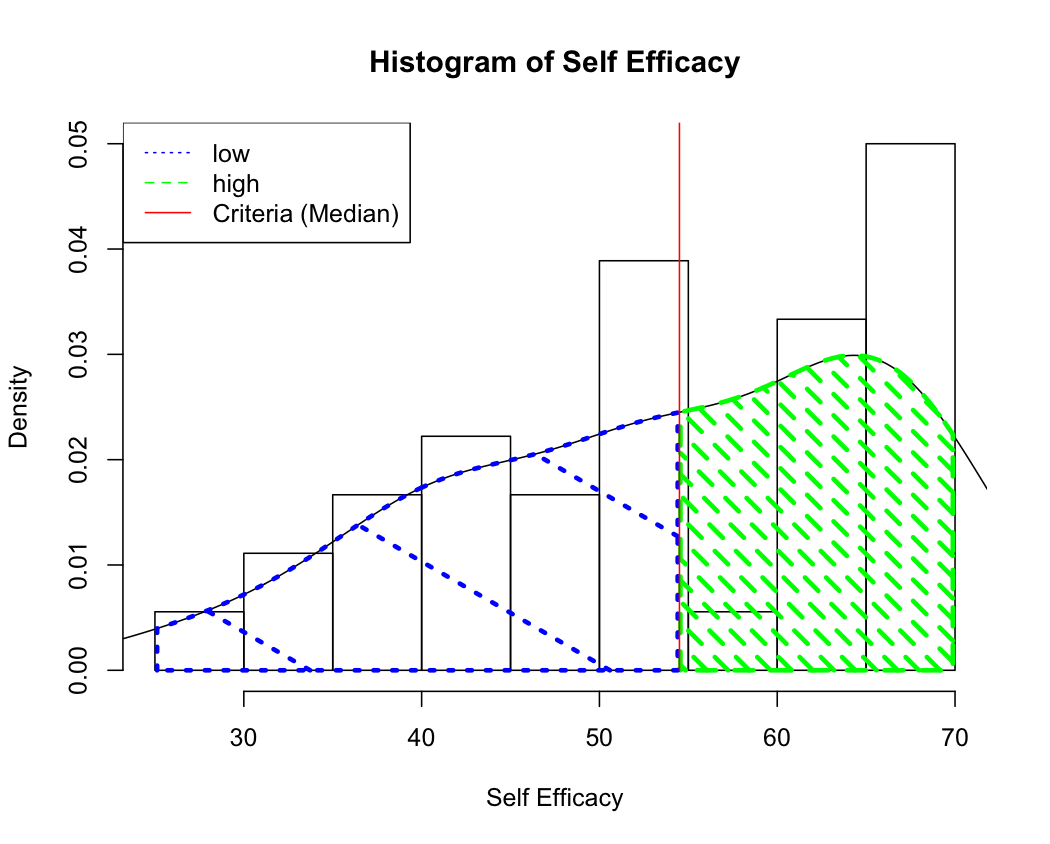
\includegraphics[width=0.9\columnwidth]{figures/hist1}
  \caption{Dirstribution of self-efficacy points and changing self-efficacy points into  factor levels low and high }~\label{fig:figure1}
\end{figure}

Then, we sort the 2 groups of 18 participants in increasing order separately by the sum of pair programming experience scores, and treat the top 9 of the participants in each group have bad pair programming experience, while the rest 9 of each group have good pair programming experience as shown in Fig.~\ref{fig:figure2}. 

\begin{figure}
\centering
  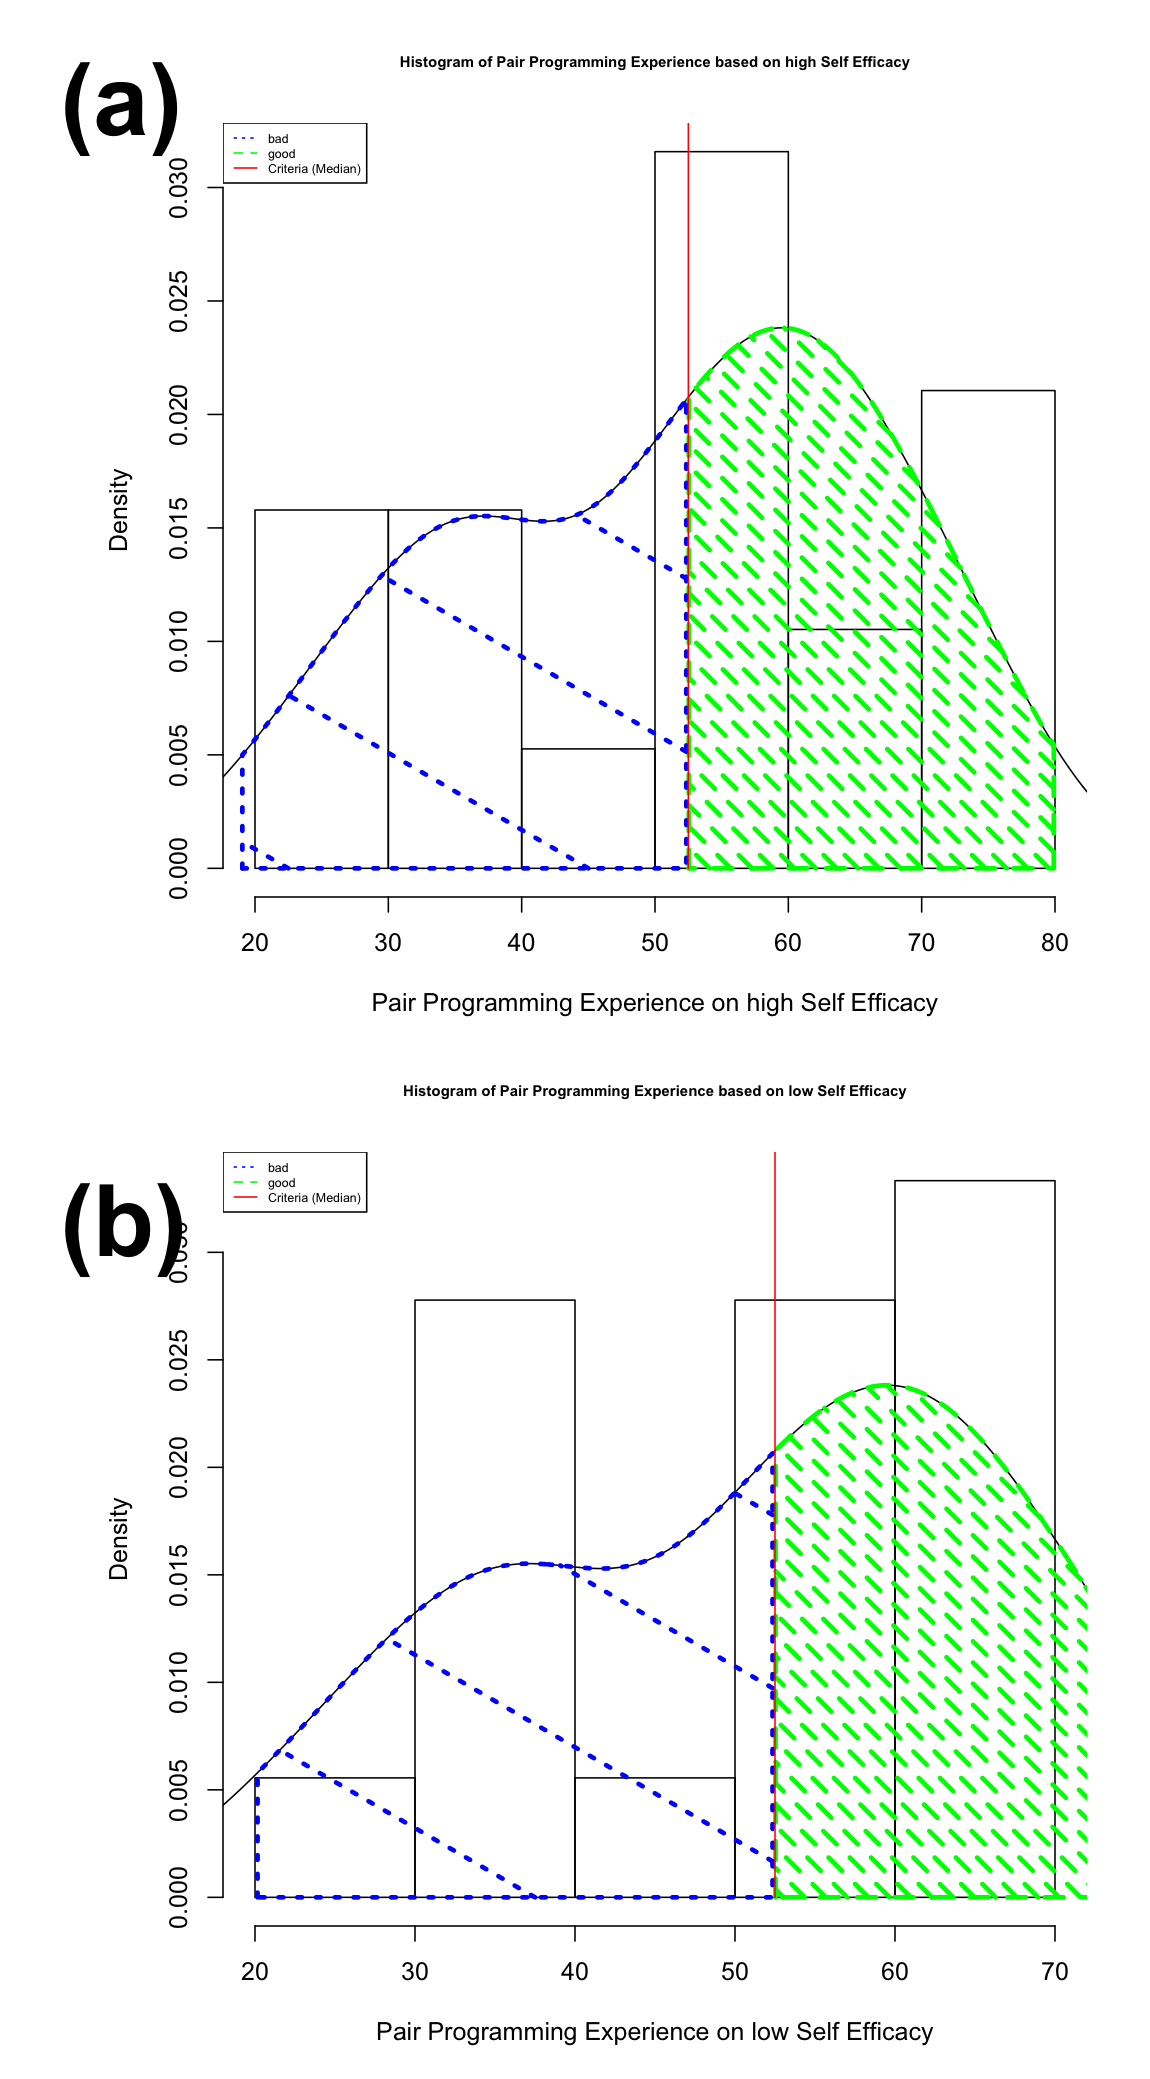
\includegraphics[width=0.8\columnwidth]{figures/hist2}
  \caption{(a)Dirstribution of pair programming experience points in high self-efficacy group and changing pair programming experience points  into  factor levels bad and good.(b)Dirstribution of pair programming experience points in low self-efficacy group and changing pair programming experience points  into  factor levels bad and good }~\label{fig:figure2}
\end{figure}




\section{Results}

Now, we get a 2x2 factorial design dataset, where the first treatment is self-efficacy with 2 levels: low and high, while the second treatment is pair programming experience with 2 levels: bad, good. Within each small block, there are 9 participants. What we can do next is to make 2 barplots for the 2 treatments, and get some general information from the barplots.

\begin{figure}
\centering
  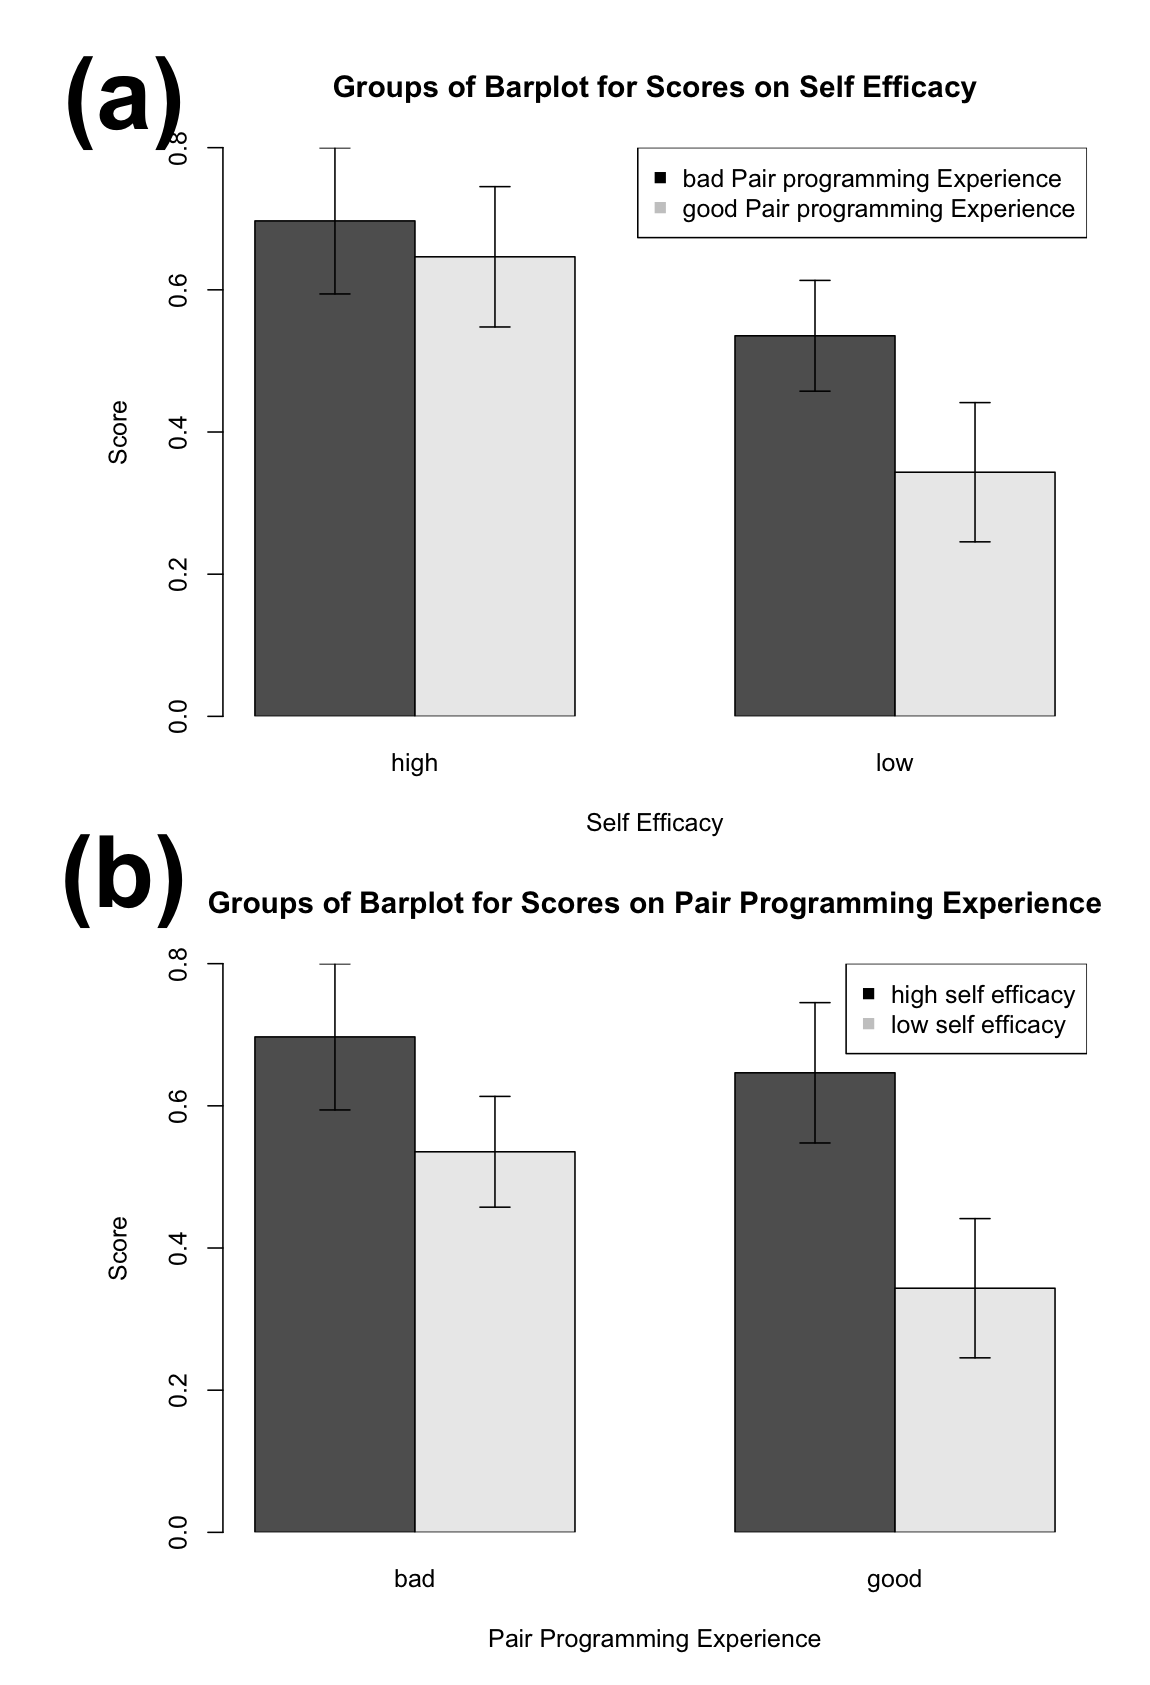
\includegraphics[width=0.8\columnwidth]{figures/fig3}
  \caption{(a)Barplots for scores on self efficacy groups. (b)Barplots for scores on pair programing experience groups.}~\label{fig:figure3}
\end{figure}

According to the Fig.~\ref{fig:figure3}, we can see that the each subgroup has similar standard error. Besides, people who have relatively bad pair programming experience get higher score no matter their self efficacy is high or low, while high self efficacy results in high score. 

After we get some sense about the main effects of the model, our next step is to make a general plot to see whether there is any potential interaction between the 2 treatments, Self Efficacy, and Pair Programming Experience, and the visualizations are shown as in Fig.~\ref{fig:figure4}

\begin{figure}
\centering
  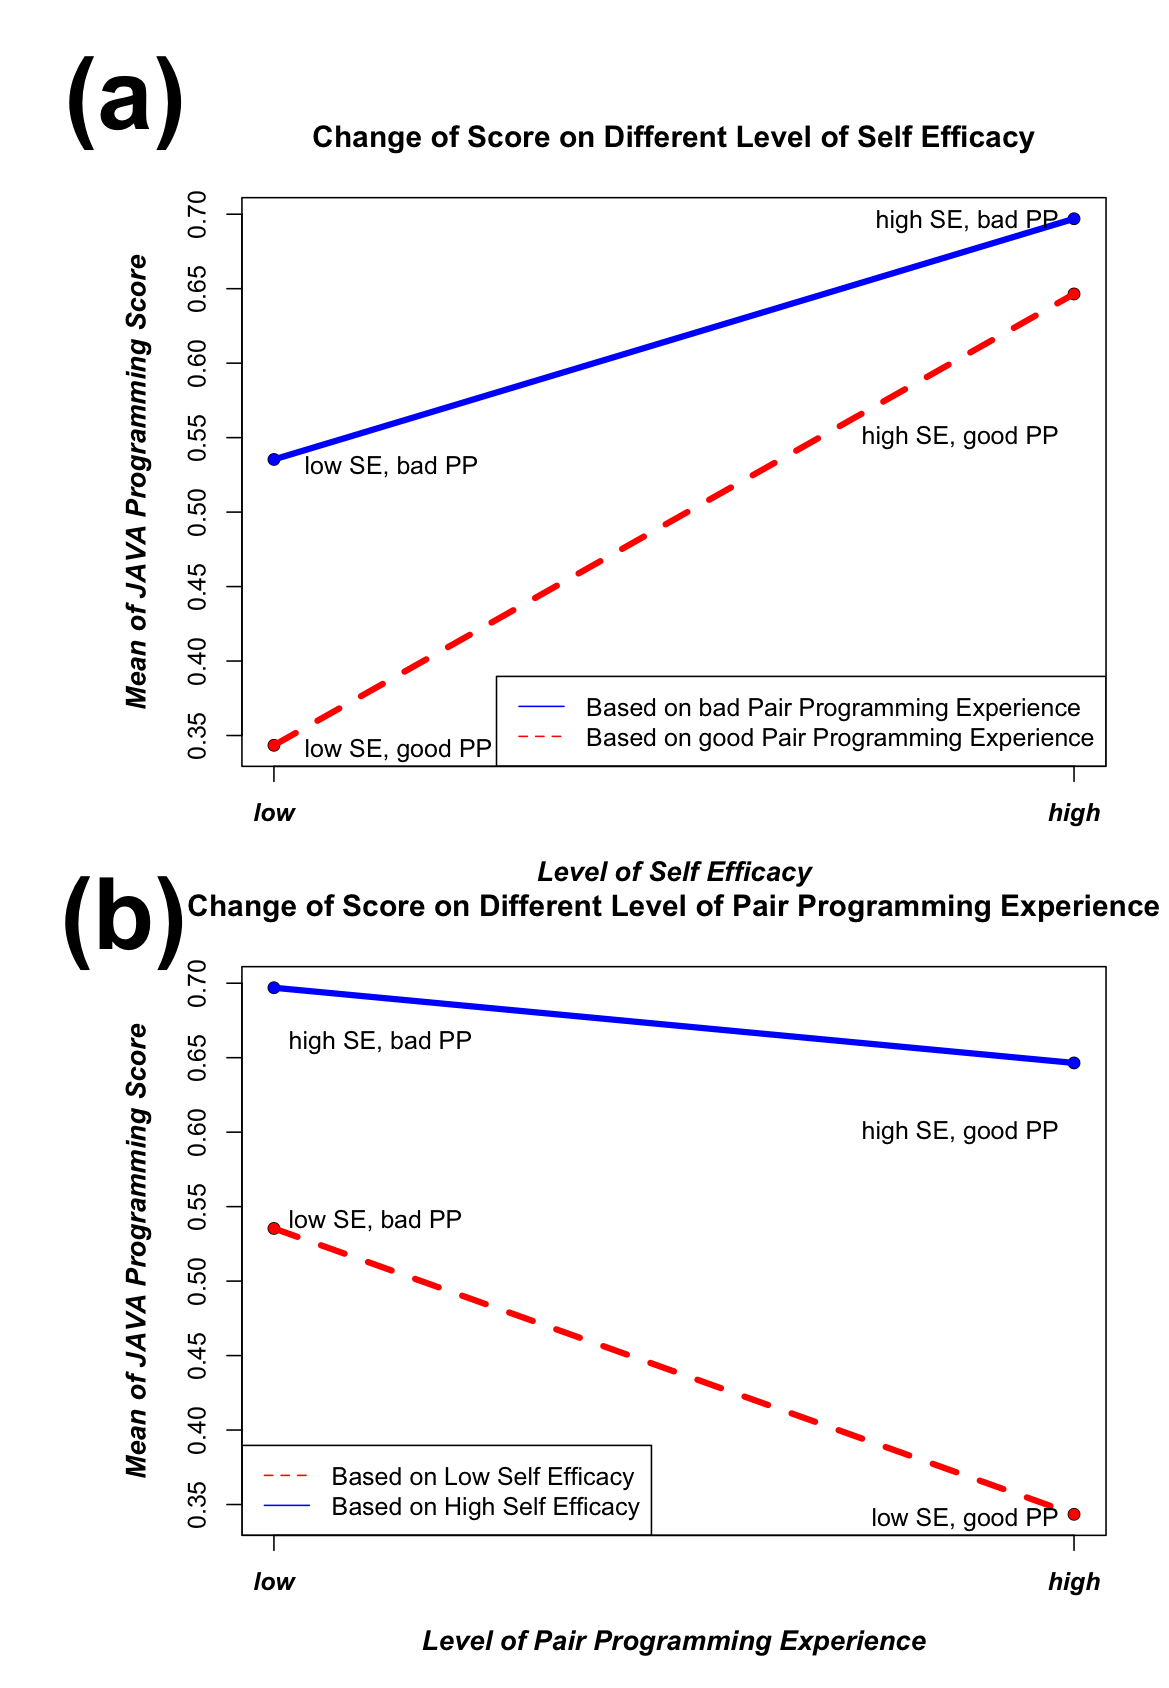
\includegraphics[width=0.8\columnwidth]{figures/fig4}
  \caption{(a)Influence of different self-efficacy levels. (b) Influence of different levels of pair programing.}~\label{fig:figure4}
\end{figure}

According to the interaction detecting plots in Fig.~\ref{fig:figure4}, there is no obvious interaction existed in any of the graph. Besides, the interaction plots show the same result as bar plot, where no matter self-efficacy is high or low, people with worse pair programming experience have higher score, and no matter pair programming experience is good or bad, higher self-efficacy leads to better scores.

Now, after some general view of the main effects and interaction effects, we calculate the ANOVA table to get a more precise test. The result is shown in Table. ~\ref{table1} .

\begin{table}[ht]
\begin{center}
\caption{ANOVA Table}
\label{table1}
\begin{tabular}{lrrrrc}
  \hline
 & Df & Sum Sq & Mean Sq & F value & Pr($>$F) \\ 
  \hline
SE      &1	&0.4858	&0.4858	 &6.003	  &~~0.0199$^*$  \\
PPE         &1	&0.1322	&0.1322	 &1.634	  &0.2103      \\ 
 SE \& PPE          &1	&0.045	&0.045	&0.556	&0.4613  \\
  Residuals  	&32	&2.5895 & 0.0809 &  &  \\ 
   \hline
   \hline
\multicolumn{6}{l}{Signif. codes    0 \textbf{ *** } 0.001 \textbf{ ** } 0.01\textbf{ * } 0.05 \textbf{ . } 0.1 \textbf{   } 1} \\ 
\hline \\
\multicolumn{6}{l}{\small SE : self-efficacy; PPE :  pair programming experience} \\
\multicolumn{6}{l}{\small SE \& PPE  : interactions between self-efficacy and pair programming experience.}
\end{tabular}
\end{center}
\end{table}

Based on the ANOVA table above, we can see that we only have weak evidence to say that the self-efficacy level does have positive influence on Java programming scores, which means that we have weak evidence to say that the higher the level of self-efficacy, the better the learning result of CS elementary programming courses. As for the experience of pair programming or the interaction effect of pair programming experience and self-efficacy level, we do not have any evidence to say they have influence on the learning result of CS elementary programming courses.

The result here partly fit our hypothesis. 


\section{Discussion}

Sample deviation in this project is not large enough probably because we selected snowball sampling for research convenience. As a result, majority of the participants were our friends and classmates. Another limitation in this research could be that some prerequisites of pair programming are not met.  For instance, students work in pairs should have a similar level of knowledge and they must obey pair programming rules such as switching roles frequently. In addition, Some participants who have a more advanced background usually do not rely on pair programming to gain programming experience. For them,  individual learning process is efficient and effective enough. Finally, pair programming may lead to good code but not good quiz performance, the latter one which is more dependent on people's exam ability difference.


\section{Conclusion}
Our study focuses on testing the main effects and interaction effects of self-efficacy level and pair programming experience to the learning result of CS elementary programming courses. We conducted a 2 x 2 factorial design for the design, and we find out that self-efficacy is the only significant factor that influencing the final learning results, whereas pair programming experience and the interaction effects of self-efficacy and pair programming experience have no significant influence on the final learning results.


%\section{Page Size and Columns}
%On each page your material should fit within a rectangle of 7 $\times$
%9.15 inches (18 $\times$ 23.2 cm), centered on a US Letter page (8.5
%$\times$ 11 inches), beginning 0.85 inches (1.9 cm) from the top of
%the page, with a 0.3 inches (0.85 cm) space between two 3.35 inches
%(8.4 cm) columns. Right margins should be justified, not
%ragged. Please be sure your document and PDF are US letter and not A4.
%
%\section{Typeset Text}
%The styles contained in this document have been modified from the
%default styles to reflect ACM formatting conventions. For example,
%content paragraphs like this one are formatted using the Normal style.
%
%\LaTeX\ sometimes will create overfull lines that extend into columns.
%To attempt to combat this, the \texttt{.cls} file has a command,
%\texttt{{\textbackslash}sloppy}, that essentially asks \LaTeX\ to
%prefer underfull lines with extra whitespace.  For more details on
%this, and info on how to control it more finely, check out
%{\url{http://www.economics.utoronto.ca/osborne/latex/PMAKEUP.HTM}}.
%
%\subsection{Title and Authors}
%
%Your paper's title, authors and affiliations should run across the
%full width of the page in a single column 17.8 cm (7 in.) wide.  The
%title should be in Helvetica or Arial 18-point bold.  Authors' names
%should be in Times New Roman or Times Roman 12-point bold, and
%affiliations in 12-point regular.  
%
%See \texttt{{\textbackslash}author} section of this template for
%instructions on how to format the authors. For more than three
%authors, you may have to place some address information in a footnote,
%or in a named section at the end of your paper. Names may optionally
%be placed in a single centered row instead of at the top of each
%column. Leave one 10-point line of white space below the last line of
%affiliations.
%
%\subsection{Abstract and Keywords}
%
%Every submission should begin with an abstract of about 150 words,
%followed by a set of Author Keywords and ACM Classification
%Keywords. The abstract and keywords should be placed in the left
%column of the first page under the left half of the title. The
%abstract should be a concise statement of the problem, approach, and
%conclusions of the work described. It should clearly state the paper's
%contribution to the field of HCI\@.
%
%\subsection{Normal or Body Text}
%
%Please use a 10-point Times New Roman or Times Roman font or, if this
%is unavailable, another proportional font with serifs, as close as
%possible in appearance to Times Roman 10-point. Other than Helvetica
%or Arial headings, please use sans-serif or non-proportional fonts
%only for special purposes, such as source code text.
%
%\subsection{First Page Copyright Notice}
%This template include a sample ACM copyright notice at the bottom of
%page 1, column 1.  Upon acceptance, you will be provided with the
%appropriate copyright statement and unique DOI string for publication.
%Accepted papers will be distributed in the conference
%publications. They will also be placed in the ACM Digital Library,
%where they will remain accessible to thousands of researchers and
%practitioners worldwide. See
%\url{http://acm.org/publications/policies/copyright_policy} for the
%ACM's copyright and permissions policy.
%
%\subsection{Subsequent Pages}
%
%On pages beyond the first, start at the top of the page and continue
%in double-column format.  The two columns on the last page should be
%of equal length.



%\subsection{References and Citations}
%
%Use a numbered list of references at the end of the article, ordered
%alphabetically by last name of first author, and referenced by numbers
%in
%brackets~\cite{acm_categories,ethics,Klemmer:2002:WSC:503376.503378}.
%Your references should be published materials accessible to the
%public. Internal technical reports may be cited only if they are
%easily accessible (i.e., you provide the address for obtaining the
%report within your citation) and may be obtained by any reader for a
%nominal fee. Proprietary information may not be cited. Private
%communications should be acknowledged in the main text, not referenced
%(e.g., ``[Borriello, personal communication]'').
%
%References should be in ACM citation format:
%\url{http://acm.org/publications/submissions/latex_style}. This
%includes citations to internet
%resources~\cite{acm_categories,cavender:writing,CHINOSAUR:venue,psy:gangnam}
%according to ACM format, although it is often appropriate to include
%URLs directly in the text, as above.


% Use a numbered list of references at the end of the article, ordered
% alphabetically by first author, and referenced by numbers in
% brackets~\cite{ethics, Klemmer:2002:WSC:503376.503378,
%   Mather:2000:MUT, Zellweger:2001:FAO:504216.504224}. For papers from
% conference proceedings, include the title of the paper and an
% abbreviated name of the conference (e.g., for Interact 2003
% proceedings, use \textit{Proc. Interact 2003}). Do not include the
% location of the conference or the exact date; do include the page
% numbers if available. See the examples of citations at the end of this
% document. Within this template file, use the \texttt{References} style
% for the text of your citation.

% Your references should be published materials accessible to the
% public.  Internal technical reports may be cited only if they are
% easily accessible (i.e., you provide the address for obtaining the
% report within your citation) and may be obtained by any reader for a
% nominal fee.  Proprietary information may not be cited. Private
% communications should be acknowledged in the main text, not referenced
% (e.g., ``[Robertson, personal communication]'').



%\begin{table}
%  \centering
%  \begin{tabular}{l r r r}
%    % \toprule
%    & & \multicolumn{2}{c}{\small{\textbf{Test Conditions}}} \\
%    \cmidrule(r){3-4}
%    {\small\textit{Name}}
%    & {\small \textit{First}}
%      & {\small \textit{Second}}
%    & {\small \textit{Final}} \\
%    \midrule
%    Marsden & 223.0 & 44 & 432,321 \\
%    Nass & 22.2 & 16 & 234,333 \\
%    Borriello & 22.9 & 11 & 93,123 \\
%    Karat & 34.9 & 2200 & 103,322 \\
%    % \bottomrule
%  \end{tabular}
%  \caption{Table captions should be placed below the table. We
%    recommend table lines be 1 point, 25\% black. Minimize use of
%    table grid lines.}~\label{tab:table1}
%\end{table}

%\section{Sections}
%
%The heading of a section should be in Helvetica or Arial 9-point bold,
%all in capitals. Sections should \textit{not} be numbered.
%
%\subsection{Subsections}
%
%Headings of subsections should be in Helvetica or Arial 9-point bold
%with initial letters capitalized.  For sub-sections and
%sub-subsections, a word like \emph{the} or \emph{of} is not
%capitalized unless it is the first word of the heading.
%
%\subsubsection{Sub-subsections}
%
%Headings for sub-subsections should be in Helvetica or Arial 9-point
%italic with initial letters capitalized.  Standard
%\texttt{{\textbackslash}section}, \texttt{{\textbackslash}subsection},
%and \texttt{{\textbackslash}subsubsection} commands will work fine in
%this template.
%
%\section{Figures/Captions}
%
%Place figures and tables at the top or bottom of the appropriate
%column or columns, on the same page as the relevant text (see
%Figure~\ref{fig:figure1}). A figure or table may extend across both
%columns to a maximum width of 17.78 cm (7 in.).

%\begin{figure*}
%  \centering
%  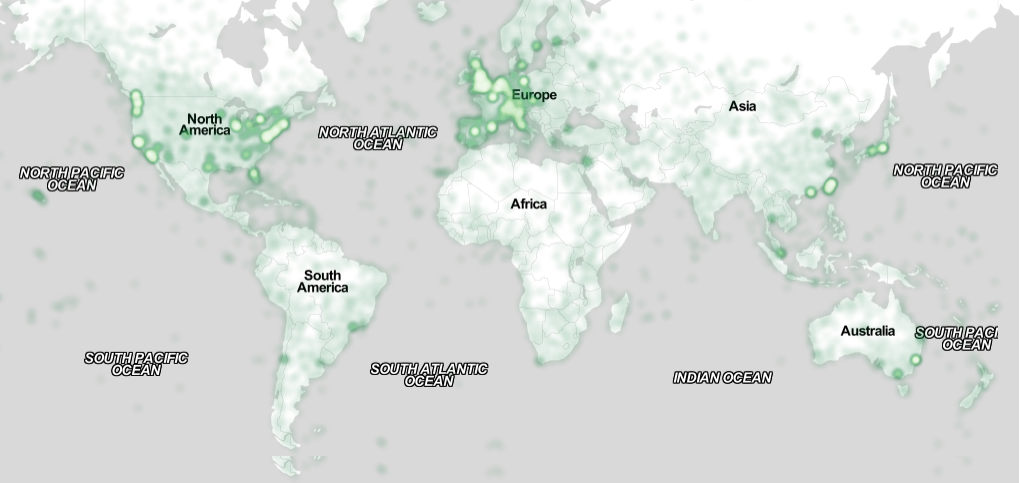
\includegraphics[width=1.75\columnwidth]{figures/map}
%  \caption{In this image, the map maximizes use of space. You can make
%    figures as wide as you need, up to a maximum of the full width of
%    both columns. Note that \LaTeX\ tends to render large figures on a
%    dedicated page. Image: \ccbynd~ayman on
%    Flickr.}~\label{fig:figure2}
%\end{figure*}

%Captions should be Times New Roman or Times Roman 9-point bold.  They
%should be numbered (e.g., ``Table~\ref{tab:table1}'' or
%``Figure~\ref{fig:figure1}''), centered and placed beneath the figure
%or table.  Please note that the words ``Figure'' and ``Table'' should
%be spelled out (e.g., ``Figure'' rather than ``Fig.'') wherever they
%occur. Figures, like Figure~\ref{fig:figure2}, may span columns and
%all figures should also include alt text for improved accessibility.
%Papers and notes may use color figures, which are included in the page
%limit; the figures must be usable when printed in black-and-white in
%the proceedings.
%
%The paper may be accompanied by a short video figure up to five
%minutes in length. However, the paper should stand on its own without
%the video figure, as the video may not be available to everyone who
%reads the paper.  

%\subsection{Inserting Images}
%When possible, include a vector formatted graphic (i.e. PDF or EPS).
%When including bitmaps,  use an image editing tool to resize the image
%at the appropriate printing resolution (usually 300 dpi).

%\section{Quotations}
%Quotations may be italicized when \textit{``placed inline''} (Anab,
%23F).



%\section{Language, Style, and Content}
%
%The written and spoken language of SIGCHI is English. Spelling and
%punctuation may use any dialect of English (e.g., British, Canadian,
%US, etc.) provided this is done consis- tently. Hyphenation is
%optional. To ensure suitability for an international audience, please
%pay attention to the following:
%
%\begin{itemize}
%\item Write in a straightforward style.
%\item Try to avoid long or complex sentence structures.
%\item Briefly define or explain all technical terms that may be
%  unfamiliar to readers.
%\item Explain all acronyms the first time they are used in your
%  text---e.g., ``Digital Signal Processing (DSP)''.
%\item Explain local references (e.g., not everyone knows all city
%  names in a particular country).
%\item Explain ``insider'' comments. Ensure that your whole audience
%  understands any reference whose meaning you do not describe (e.g.,
%  do not assume that everyone has used a Macintosh or a particular
%  application).
%\item Explain colloquial language and puns. Understanding phrases like
%  ``red herring'' may require a local knowledge of English.  Humor and
%  irony are difficult to translate.
%\item Use unambiguous forms for culturally localized concepts, such as
%  times, dates, currencies, and numbers (e.g., ``1--5--97'' or
%  ``5/1/97'' may mean 5 January or 1 May, and ``seven o'clock'' may
%  mean 7:00 am or 19:00). For currencies, indicate equivalences:
%  ``Participants were paid {\fontfamily{txr}\selectfont \textwon}
%  25,000, or roughly US \$22.''
%\item Be careful with the use of gender-specific pronouns (he, she)
%  and other gendered words (chairman, manpower, man-months). Use
%  inclusive language that is gender-neutral (e.g., she or he, they,
%  s/he, chair, staff, staff-hours, person-years). See the
%  \textit{Guidelines for Bias-Free Writing} for further advice and
%  examples regarding gender and other personal
%  attributes~\cite{Schwartz:1995:GBF}. Be particularly aware of
%  considerations around writing about people with disabilities.
%\item If possible, use the full (extended) alphabetic character set
%  for names of persons, institutions, and places (e.g.,
%  Gr{\o}nb{\ae}k, Lafreni\'ere, S\'anchez, Nguy{\~{\^{e}}}n,
%  Universit{\"a}t, Wei{\ss}enbach, Z{\"u}llighoven, \r{A}rhus, etc.).
%  These characters are already included in most versions and variants
%  of Times, Helvetica, and Arial fonts.
%\end{itemize}

%\section{Accessibility}
%The Executive Council of SIGCHI has committed to making SIGCHI
%conferences more inclusive for researchers, practitioners, and
%educators with disabilities. As a part of this goal, the all authors
%are asked to work on improving the accessibility of their
%submissions. Specifically, we encourage authors to carry out the
%following five steps:
%\begin{enumerate}
%\item Add alternative text to all figures
%\item Mark table headings
%\item Add tags to the PDF
%\item Verify the default language
%\item Set the tab order to ``Use Document Structure''
%\end{enumerate}
%For more information and links to instructions and resources, please
%see: \url{http://chi2016.acm.org/accessibility}.  The
%\texttt{{\textbackslash}hyperref} package allows you to create well tagged PDF files,
%please see the preamble of this template for an example.
%
%\section{Page Numbering, Headers and Footers}
%Your final submission should not contain footer or header information
%at the top or bottom of each page. Specifically, your final submission
%should not include page numbers. Initial submissions may include page
%numbers, but these must be removed for camera-ready. Page numbers will
%be added to the PDF when the proceedings are assembled.
%
%\section{Producing and Testing PDF Files}
%
%We recommend that you produce a PDF version of your submission well
%before the final deadline.  Your PDF file must be ACM DL
%Compliant. The requirements for an ACM Compliant PDF are available at:
%{\url{http://www.sheridanprinting.com/typedept/ACM-distilling-settings.htm}}.
%
%Test your PDF file by viewing or printing it with the same software we
%will use when we receive it, Adobe Acrobat Reader Version 10. This is
%widely available at no cost. Note that most
%reviewers will use a North American/European version of Acrobat
%reader, so please check your PDF accordingly.
%
%When creating your PDF from Word, ensure that you generate a tagged
%PDF from improved accessibility. This can be done by using the Adobe
%PDF add-in, also called PDFMaker. Select Acrobat | Preferences from
%the ribbon and ensure that ``Enable Accessibility and Reflow with
%tagged Adobe PDF'' is selected. You can then generate a tagged PDF by
%selecting ``Create PDF'' from the Acrobat ribbon.


\section{Acknowledgments}

We thank all the volunteers, and all publications support, classmates  and staff, who wrote and provided helpful comments on previous versions of this document. 
We especially want to thank Prof. Mutlu for instructing our whole design of this study,  Prof. Legault for helping us preparing the questionnaire and Prof. Deppeler for helping us recruiting the volutenners in CS 367.
We would like to thank Prof. Barbara Ericson at Georgia Tech for the Java questions we used from hera wonderful Java Review Website\footnote{\url{http://interactivepython.org/runestone/static/JavaReview/index.html}}.




% Balancing columns in a ref list is a bit of a pain because you
% either use a hack like flushend or balance, or manually insert
% a column break.  http://www.tex.ac.uk/cgi-bin/texfaq2html?label=balance
% multicols doesn't work because we're already in two-column mode,
% and flushend isn't awesome, so I choose balance.  See this
% for more info: http://cs.brown.edu/system/software/latex/doc/balance.pdf
%
% Note that in a perfect world balance wants to be in the first
% column of the last page.
%
% If balance doesn't work for you, you can remove that and
% hard-code a column break into the bbl file right before you
% submit:
%
% http://stackoverflow.com/questions/2149854/how-to-manually-equalize-columns-
% in-an-ieee-paper-if-using-bibtex
%
% Or, just remove \balance and give up on balancing the last page.
%
%\balance{}
%
%\section{References Format}
%Your references should be published materials accessible to the
%public. Internal technical reports may be cited only if they are
%easily accessible and may be obtained by any reader for a nominal
%fee. Proprietary information may not be cited. Private communications
%should be acknowledged in the main text, not referenced (e.g.,
%[Golovchinsky, personal communication]). References must be the same
%font size as other body text. References should be in alphabetical
%order by last name of first author. Use a numbered list of references
%at the end of the article, ordered alphabetically by last name of
%first author, and referenced by numbers in brackets. For papers from
%conference proceedings, include the title of the paper and the name of
%the conference. Do not include the location of the conference or the
%exact date; do include the page numbers if available. 
%
%References should be in ACM citation format:
%\url{http://www.acm.org/publications/submissions/latex_style}.  This
%includes citations to Internet
%resources~\cite{CHINOSAUR:venue,cavender:writing,psy:gangnam}
%according to ACM format, although it is often appropriate to include
%URLs directly in the text, as above. Example reference formatting for
%individual journal articles~\cite{ethics}, articles in conference
%proceedings~\cite{Klemmer:2002:WSC:503376.503378},
%books~\cite{Schwartz:1995:GBF}, theses~\cite{sutherland:sketchpad},
%book chapters~\cite{winner:politics}, an entire journal
%issue~\cite{kaye:puc},
%websites~\cite{acm_categories,cavender:writing},
%tweets~\cite{CHINOSAUR:venue}, patents~\cite{heilig:sensorama}, and
%online videos~\cite{psy:gangnam} is given here.  See the examples of
%citations at the end of this document and in the accompanying
%\texttt{BibTeX} document. This formatting is a edited version of the
%format automatically generated by the ACM Digital Library
%(\url{http://dl.acm.org}) as ``ACM Ref.'' DOI and/or URL links are
%optional but encouraged as are full first names. Note that the
%Hyperlink style used throughout this document uses blue links;
%however, URLs in the references section may optionally appear in
%black.

% REFERENCES FORMAT
% References must be the same font size as other body text.
\bibliographystyle{SIGCHI-Reference-Format}
\bibliography{sample}

\end{document}

%%% Local Variables:
%%% mode: latex
%%% TeX-master: t
%%% End:
